\documentclass{article}
\usepackage{tabularx}
\usepackage[english]{babel}
\usepackage{blindtext}
\usepackage{listings}

\usepackage{graphicx} % Required for inserting images
\usepackage{array}
\renewcommand{\arraystretch}{2.5}
\title{PKS 2024 Project}
\author{Amal Akhmadinurov}
\date{November 2024}

\begin{document}

\maketitle
\tableofcontents
\newpage
\section{Introduction}


This paper provides a comprehensive description of the proposed protocol and its implementation.
Developed protocol operates at the application layers and is designed to reliably transfer data in between two hosts. The protocol supports transfer of both text and file data. To improve its reliability Selective Repeat ARQ method was implemented, which helps to retransmit lost or damaged fragments. This allows to request retransmission of only specific fragments, what seriously improves its capabilities in unreliable networks. In additions to this, the protocol incorporates both positive and negative acknowledgements, that signals successful and unsuccessful transmission of fragments. 

It is also notable that dynamic window size is implemented to increase the effectiveness of this algorithm in error-prone networks. This feature makes the protocol more flexible and allows it to be able to adapt the networks throughput.

Moreover, the protocol is designed to handle arbitrary number of fragments as well as the transmission of texts and files of different sizes.

The protocol was implemented using the C\# programming language, using only the standard .NET libraries. This choice of implementation provides compatibility with the .NET framework while maintaining simplicity and reliability in the protocol's design and execution. By relying solely on standard libraries, the implementation is both accessible and maintainable, making it easy to extend or modify in the future.



\newpage
\section{Protocol header}

\subsection{Structure}

\begin{tabular}{|p{2cm}|p{1cm}|p{1cm}|p{2cm}|p{3cm}|p{2cm}|}
\hline
Sequence Number (2b) & 
ID (2b) & 
Flags  (1b)& 
Filename Offset (2b) &
Data (0-1463b) &
Checksum (2b)

\\
\hline




\end{tabular}
\newline
\newline

\textbf{Sequence Number} is a 2 byte integer to store the number of the fragment. Used for Selective repeat ARQ method. 
\newline

\textbf{ID}  is a 2 byte integer to distinct fragments of different messages. Assigned to a random number. Main purpose of this field is to make it possible to handle fragments from several message at the same time. To distinguish between control message and fragments, ID is 0 for all control messages.
\newline

\textbf{Flags}  is a 1 byte containing the following flags (from the most significant bit to the leats significant bit):
\begin{itemize}
  \item Ack  
  \item Syn
  \item Last
  \item Keep-Alive
  \item File  
  \item Finish

 
\end{itemize}
\textbf{Ack} and \textbf{Syn} are used for setting up the initial connection as well as positive and negative acknowledgements
\newline
\textbf{Last} flags indicates the last fragment of the message.
\newline
\textbf{Keep-Alive} used for keeping connection alive.
\newline
\textbf{File} indicates file message.
\newline
\textbf{Finish} is used to terminate connection.
\newline
\textbf{Filename Offset}  is a 2 byte integer to indicate the amount of bytes in data part to be considered as filename. Ignored if File flag is 0.
\newline

\textbf{Data} contains data.
\newline

\textbf{Checksum} is a 2 byte fields containing CRC16 value to check the integrity of the message.

\subsection{Sequence Number excess}
In case more fragments will be needed than 65536 (max. values of 2 byte unsigned int) the following mechanism will be applied. After the fragment with sequence number 65535 is sent, sender will wait until all fragments will be acknowledged  to avoid possible collisions.Then it will reset sequence number to 0 and start sending new fragments. The receiver in case of excess of sequence number does not changes its behaviour as it saves every fragment with unique internal sequence number which reflects fragment position in the message, which prevents sequence numbers collisions.

\newpage
\section{Establishing and terminating connection}

\subsection{Establishing connection}
\begin{figure}[h]
    \centering
    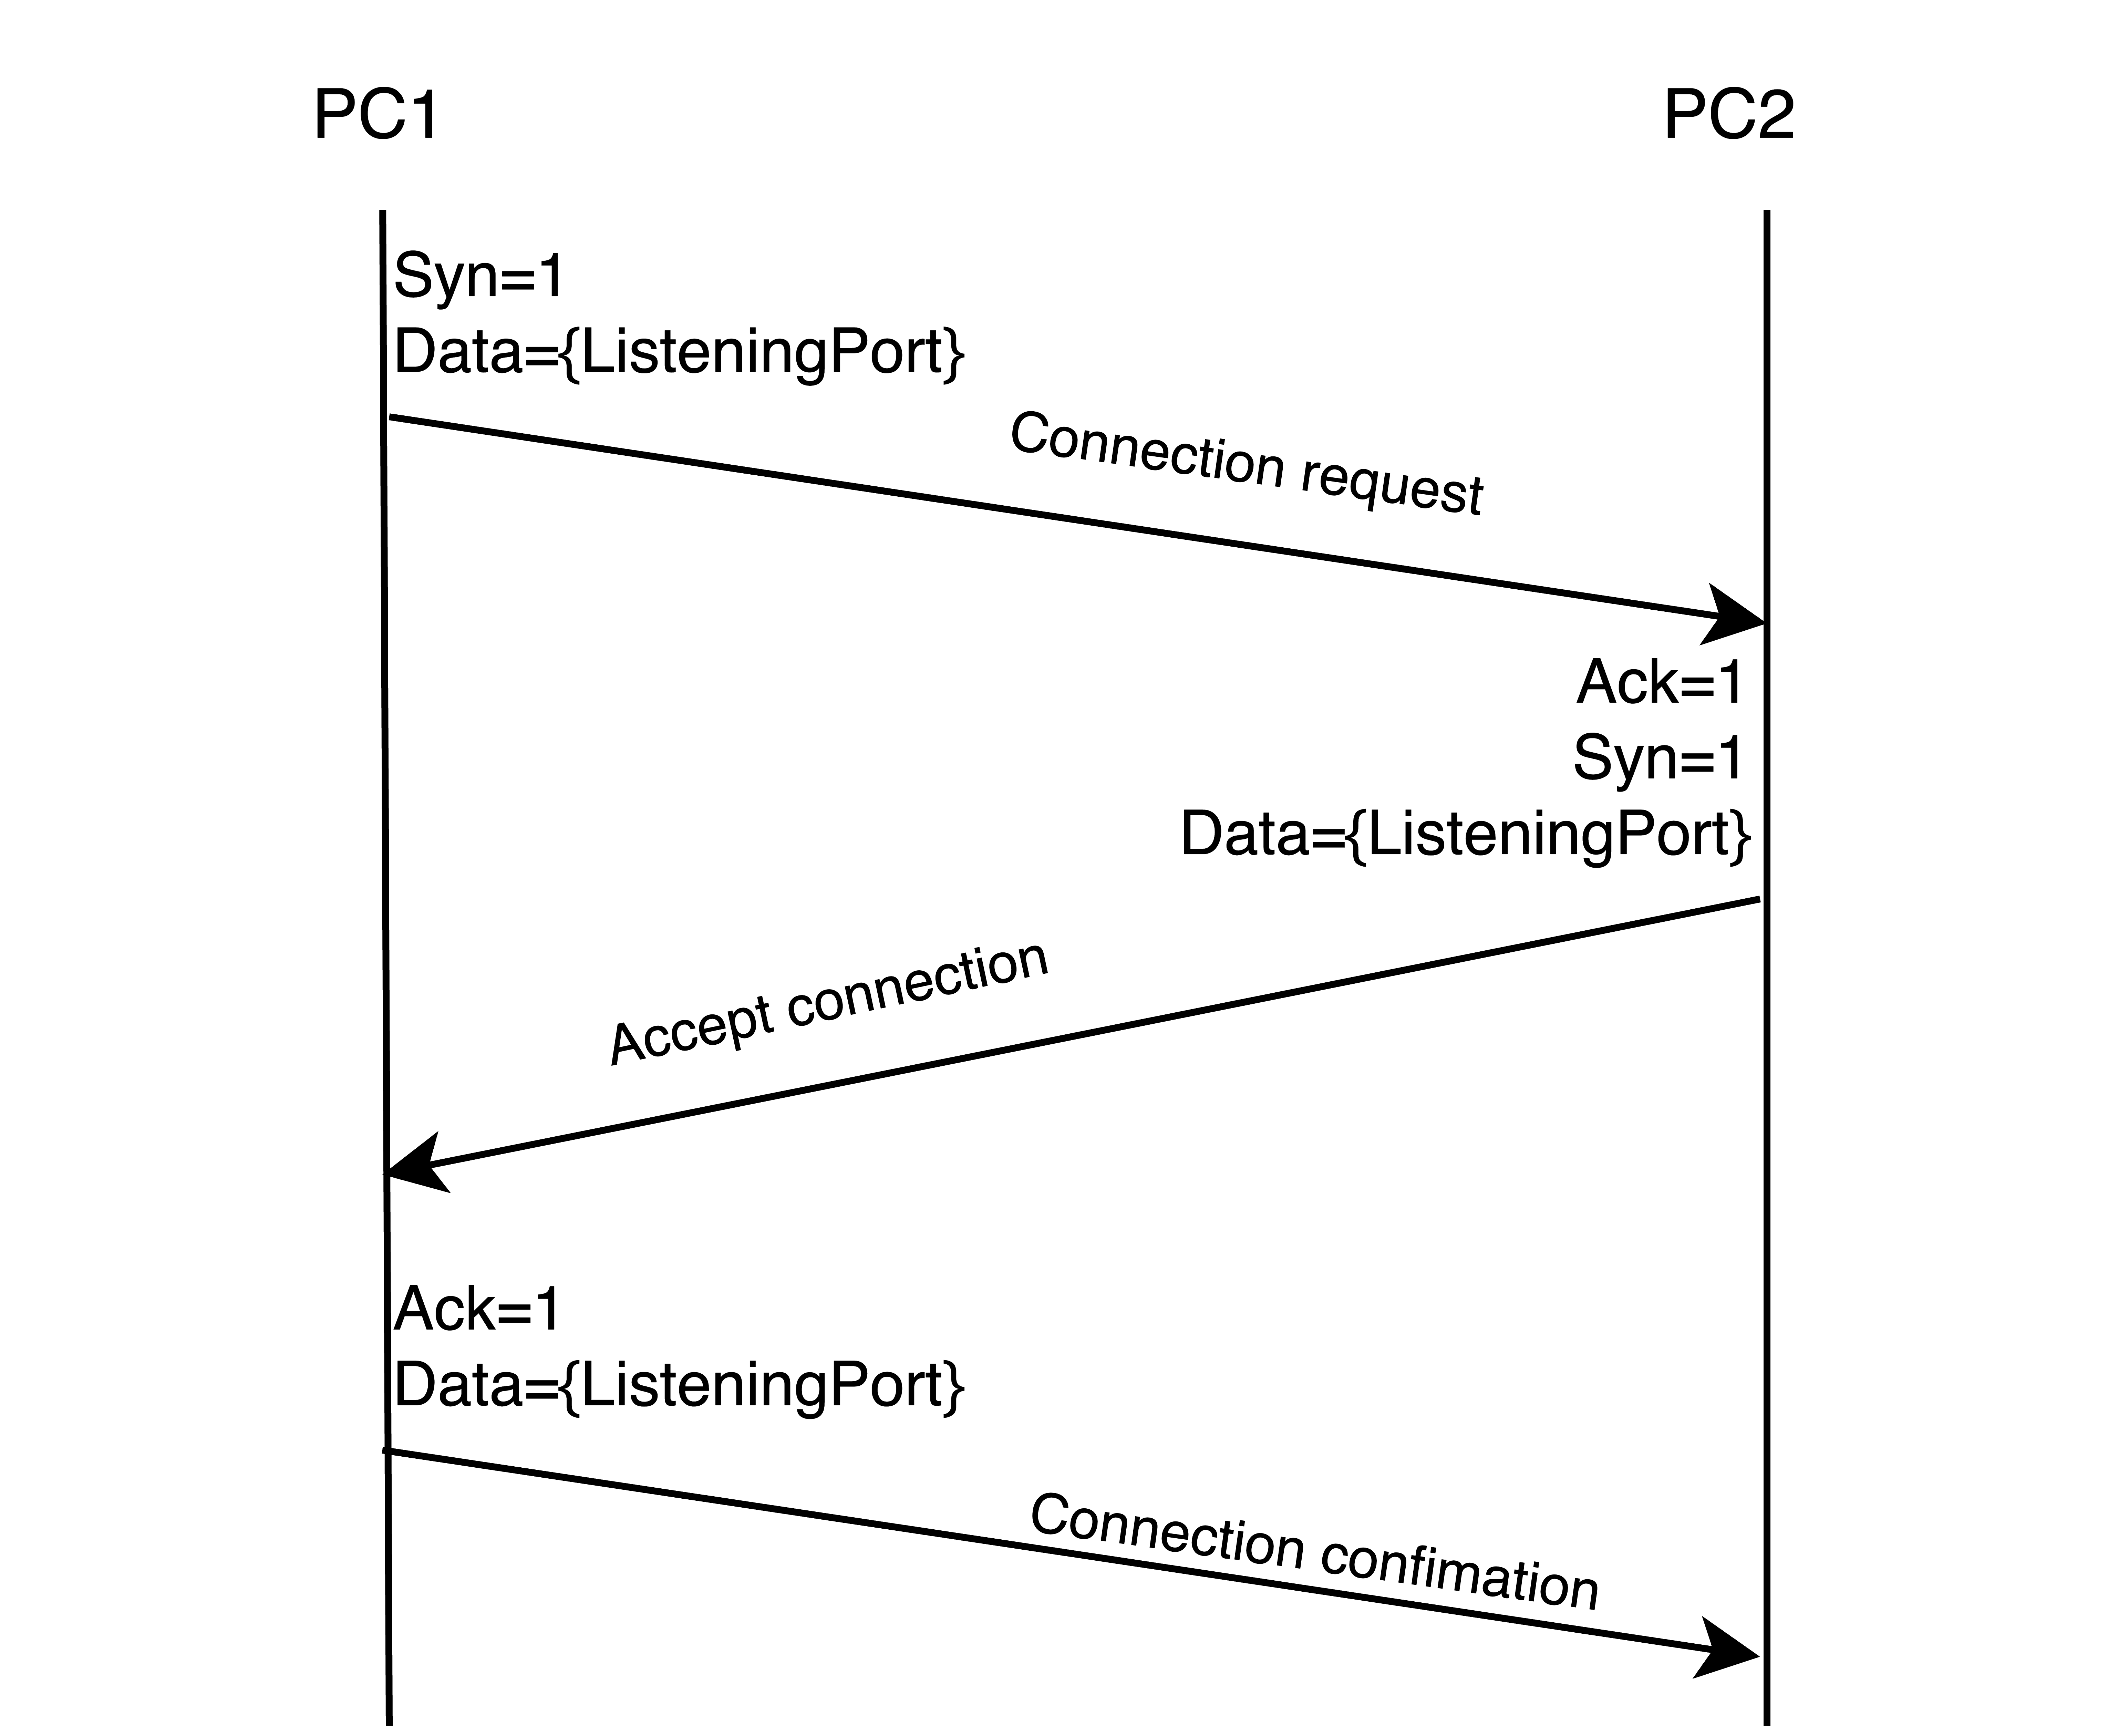
\includegraphics[width=\textwidth]{images/connection.png}
    \caption{Scheme of establishing connection}
    \label{fig:mesh1}
\end{figure}
Firstly, connection request is made (from PC1) to PC2. It contains flag Syn=1 and the listening port in Data.
\newline
PC2 responds back message indicating that  connection was accepted. This response contains flags Syn=1, Ack=1 and its own listening port as Data. PC2 now is waiting for the acknowledgement.
\newline
PC1 has to send acknowledgement , which is message with flag Ack=1.
\newline
After these steps connection is considered to be established.

\subsection{Terminating connection}

Terminating connection is done by sending request with flag Finish=1. After this connection is considered to be terminated.


\section{Keep-Alive}

\begin{figure}[h]
    \centering
    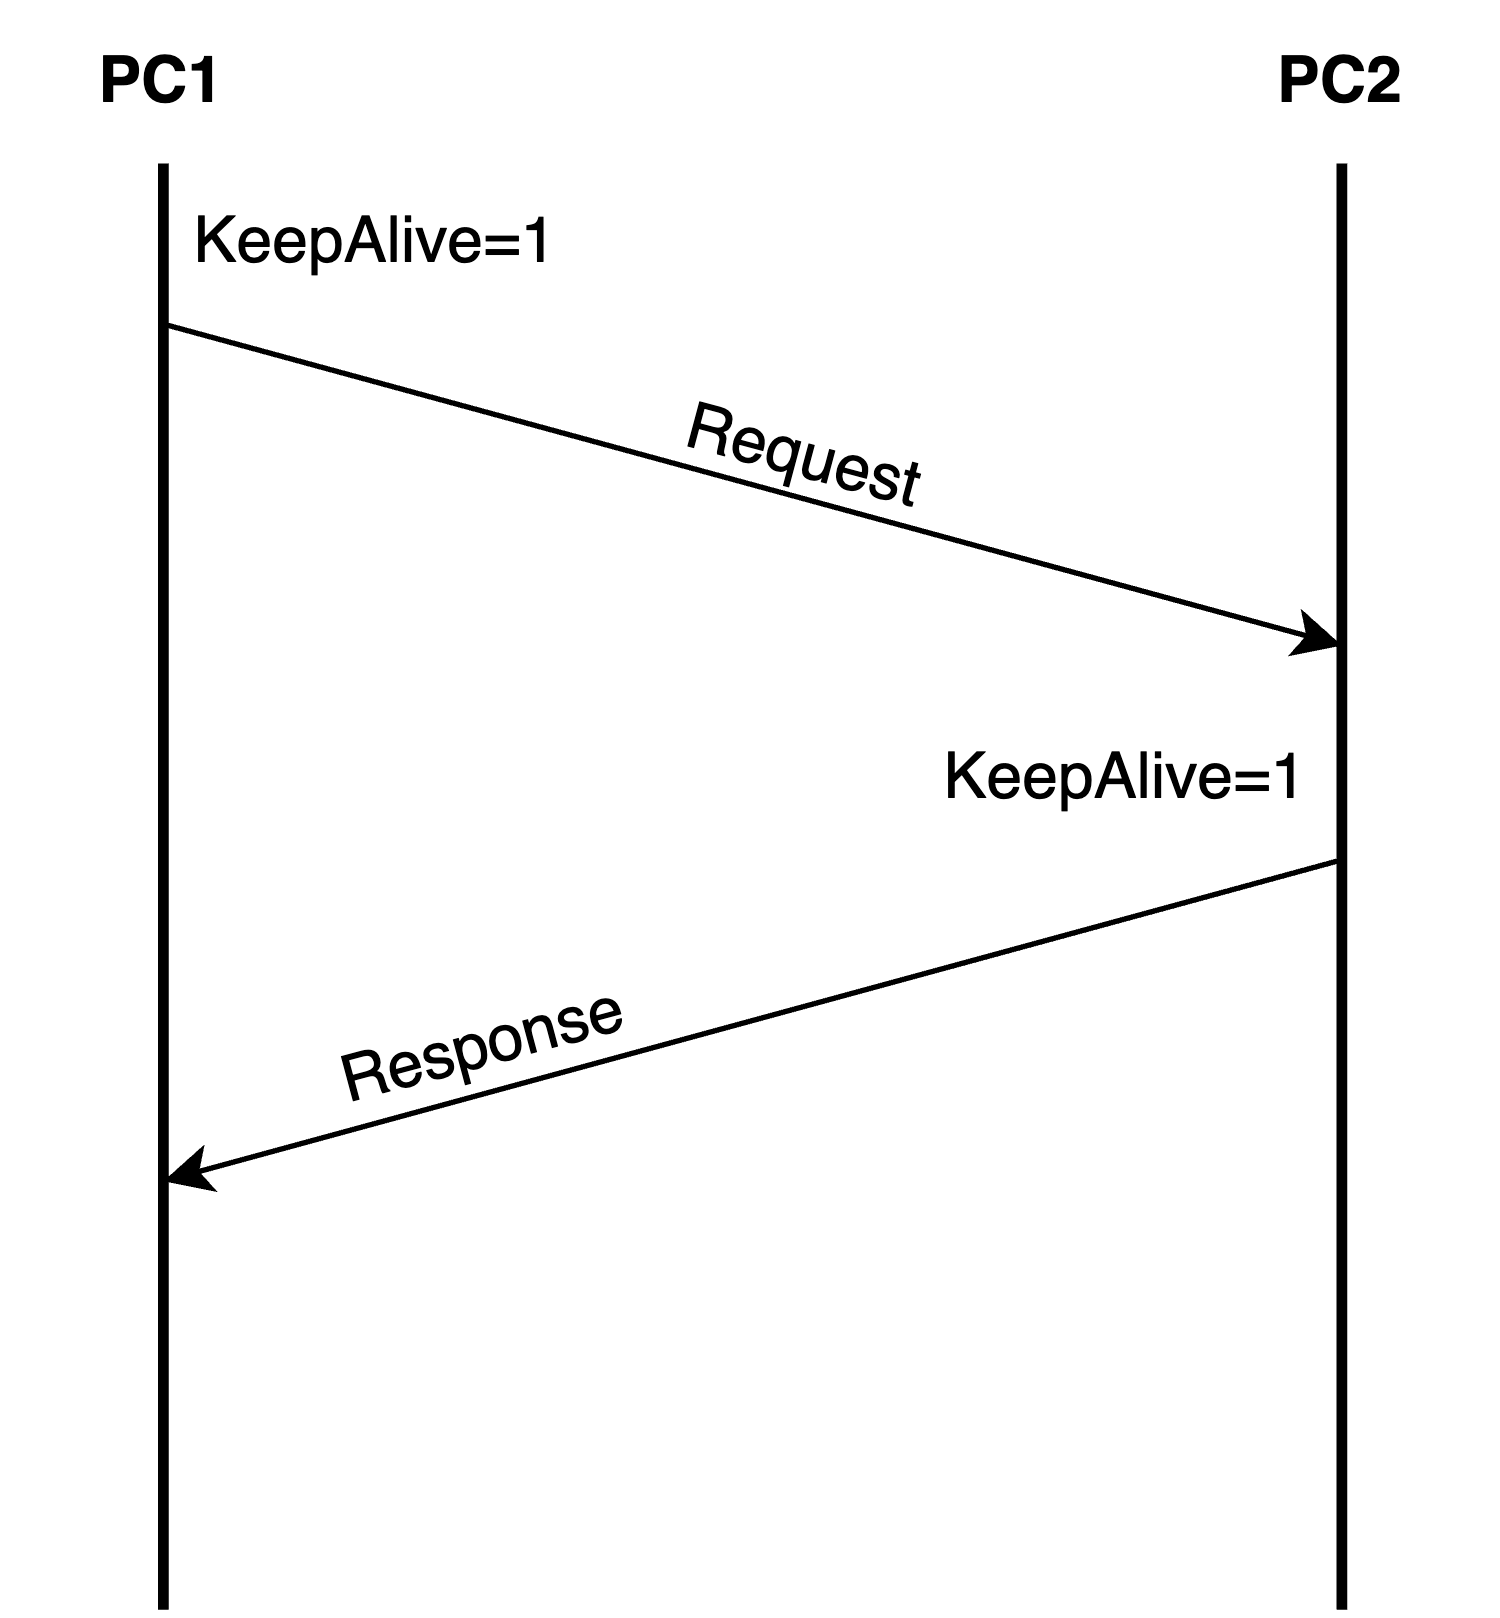
\includegraphics[width=\textwidth]{images/keepalive.png}
    \caption{Scheme of Keep-Alive requests}
    \label{fig:mesh1}
\end{figure}
To keep the connection alive special message are used. Every 5 seconds each peer sends Keep-Alive request, that is a message with flag KeepAlive=1 . The other side has to respond with the the flag KeepAlive=1 and Ack=1. After 3 consecutive unresponded "Keep-Alive" requests connection is considered to be lost and terminated. In case transmission is happening both a sender and a receiver half of a second check when the latest fragment was delivered (in case of a sender latest acknowledgement). If the latest fragment/acknowledgement was delivered more than 5 seconds ago, three consecutive "Keep alive" requests are sent and if there is no response for at least one of them connection is considered to be lost.

\newpage

\section{Error simulation}

By default messages are sent without error. To turn on error simulation special flag is used. Examples:
\begin{lstlisting}
sendtext -err
\end{lstlisting}
\begin{lstlisting}
sendfile path/to/your/file -err
\end{lstlisting}

Error simulation will always damage at least one fragment. Other fragments will be damaged randomly with small probability. Damaged are always either in data part or in checksum (as told in the assignment). Error is done by selecting random byte and assigning it to a random value.

\newpage

\section{Data integrity}


\subsection{CRC16}

To control data integrity CRC16 algorithm is used. 
Own implementation of CRC16 is used.
During the computation algorithm will go  through every byte of data to be included in the message. Initially CRC is null. It will shift current CRC value by 8 to the right and perform XOR operation between current byte and CRC. Computed value is used as index for the lookup table. Value from the table is XORed with the CRC value shifted to the left by 8. This CRC value then is used for the computation for the next byte. CRC value that is computed for the last byte is the final value to be included in the Checksum part of the message. \newline
Lookup table is only an optimisation for the whole algorithm. Assuming that byte can have only 256 values.
Table is filled with byte values after applying CRC key. Every byte is assigned to 2 byte int and shifted by 8, because CRC value is two byte value. After this the algorithm move though every bit of the byte: if the leading bit in the byte is null then it shifted by 1 to the left, if not it is shifted by 1 to the left and XORed with the value of the key. This step repeat 8 times for every byte value and the computed value put to the table, where index is the initial byte value and the value is the computed value.

\subsection{Acknowledgements}

When a receiver process new fragment, it always sends positive acknowledgement, if fragment is delivered correctly. It does not send a negative acknowledgement for the damaged fragment because theoretically an error can be in the header and the  sequence number part may be damaged and that is why it is impossible to request the right fragment again and the fragment is just discarded.

If the fragment is received successfully, a receiver always iterate back from fragment sequence number -1 until it finds the delivered fragment, sending negative acknowledgements for all undelivered fragments. By doing this it is possible to check whether previous fragments were delivered or not. It iterates until it encounter a delivered fragment, this principle reduces time of processing one fragment as previously successfully delivered fragments already checked fragments before them. While checking previous fragments, it immediately sends negative acknowledgements for every missing fragments.

Positive acknowledgement is represented by message with flag Ack=1 and the sequence number set to respective sequence number of the fragment.
Negative acknowledgement is represented by message with flag Syn=1 and the sequence number set to respective sequence number of the fragment.



\section{Selective repeat ARQ}

\subsection{Description}
Selective repeat was chosen as ARQ method. 

\begin{figure}[!h]
    \centering
    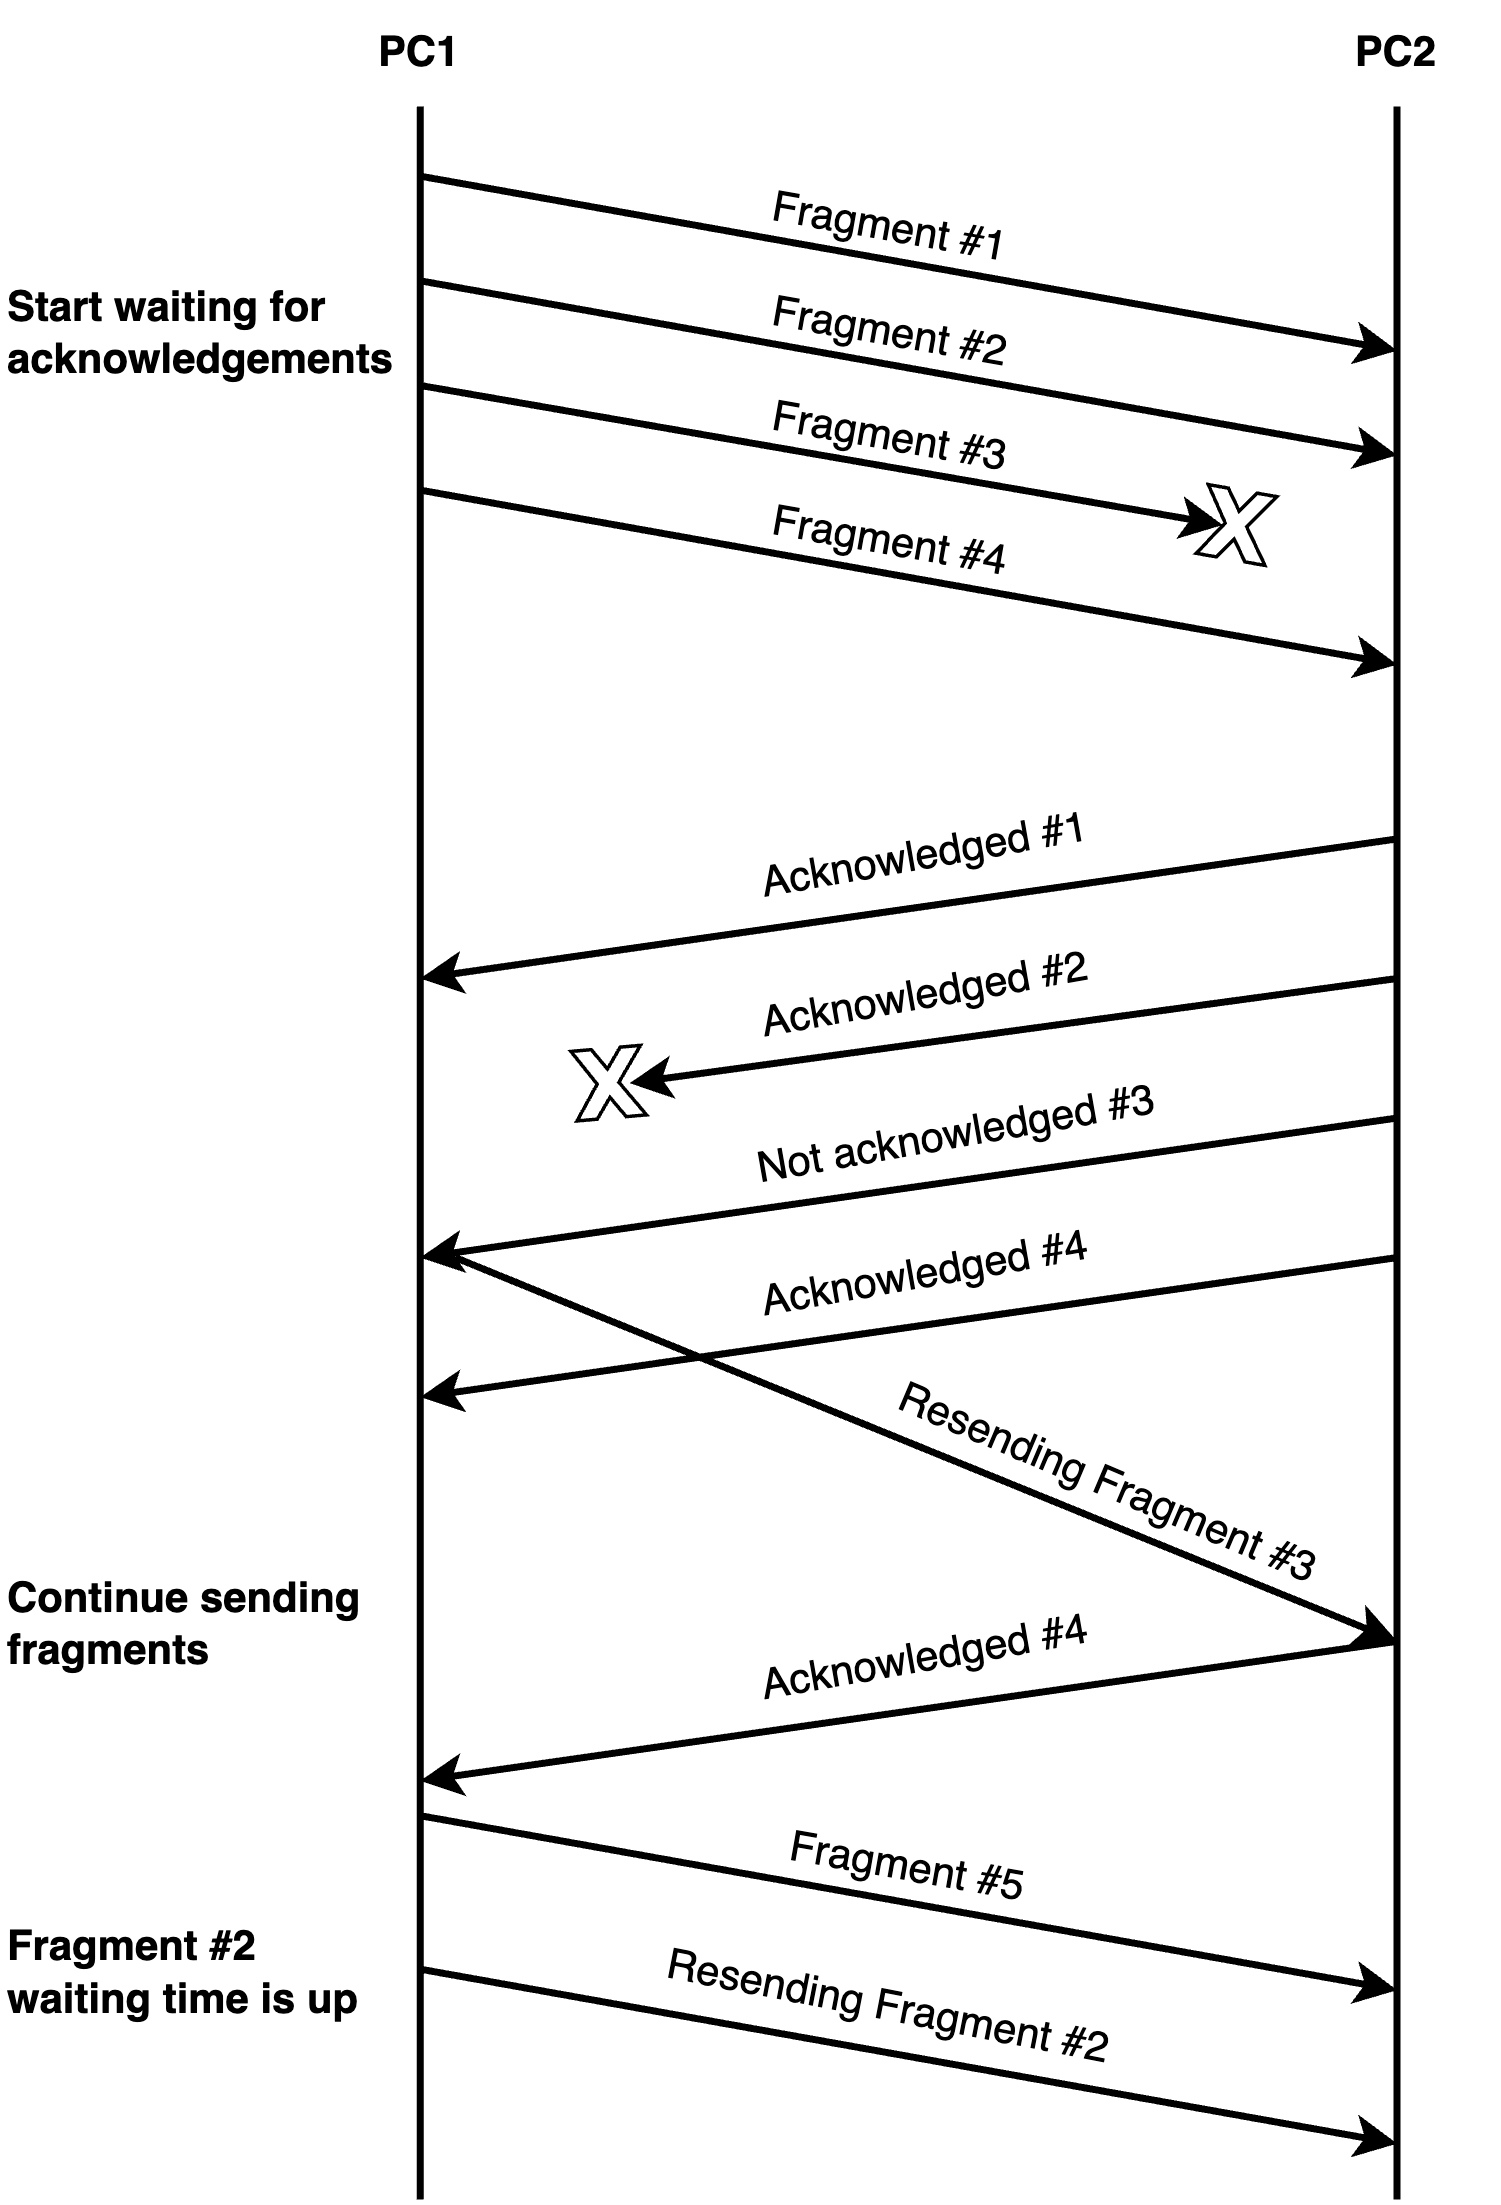
\includegraphics[width=0.75\textwidth]{images/arq.png}
    \caption{Scheme of Selective repeat ARQ for window size 4}
    \label{fig:mesh1}
\end{figure}

In the beginning, the sender sends several fragments (in this case 4, as window size is 4) without waiting for their acknowledgements, but starts timer for every fragment.  Receiver acknowledges every frame it gets. After receiving each fragment, it iterates from the current fragment sequence number minus 1 until it finds the delivered one, sending negative acknowledgements for every that was not delivered. Using this principle every fragment control previous fragments delivery    In the example shown in the Figure 3 fragment number 3 is not delivered or delivered with an error and that is why negative acknowledgement is sent. At the same time the acknowledgement for the second fragment is lost or not delivered  either.  PC1 resends fragment 3 as it received negative acknowledgement and also sends fragment 5  without waiting. After some period of time, PC1 resends fragment 2 as it didn't get acknowledgement in time.\newline
In the implementation the initial window size is 10 fragments. It is relatively small, because it has a dynamic size. Sender in the implementation waits for 2 seconds before resending fragment \newline
To acknowledge delivery of a fragment a message sent containing flag Ack=1 and a sequence number of a fragment. To send a negative acknowledgement a message contains Syn=1 and a sequence number of a fragment. In both cases ID field is set to respective ID of the message.

\subsection{Dynamic window}
As mentioned earlier, the window size is dynamic and depends on the throughput of the networks.\newline
Size is corrected in the following way. When fragment acknowledgement is received by a sender,   the time it took to get this acknowledgement is compared to the threshold value (200 milliseconds in the implementation). If the time is bigger than threshold, it reduces the window size by half, if not increases by one. Only sender knows about the current window size as a receiver just acknowledges fragment or not. 

\pagebreak

\section{Program interface}
\subsection{Compile and run}

Open Project from src directory and open in Visual Studio Code, which will suggest steps to run it. In case it did't happen do the following:
\begin{enumerate}
\item https://dotnet.microsoft.com/ru-ru/download - download .NET SDK
\item Install C\# DevKit extension for VS Code
\item Install C\# extension for VS Code
\item Try run the projects
\end{enumerate}

\subsection{Usage}
Connection to the peer
\begin{lstlisting}
connect 127.0.0.1:5050
\end{lstlisting}
Disconnection from the peer
\begin{lstlisting}
disconnect
\end{lstlisting}
Send simple text message with fragment size 10 bytes and error simulation
\begin{lstlisting}
sendtext -fs 10 -err
\end{lstlisting}
Send file with fragment size 10 bytes and error simulation
\begin{lstlisting}
sendfile path/to/your/file -fs 10 -err
\end{lstlisting}
Set path to save received files
\begin{lstlisting}
savepath path/to/your/file 
\end{lstlisting}
\newpage

\section{Diagrams}
\begin{figure}[!h]
    \centering
    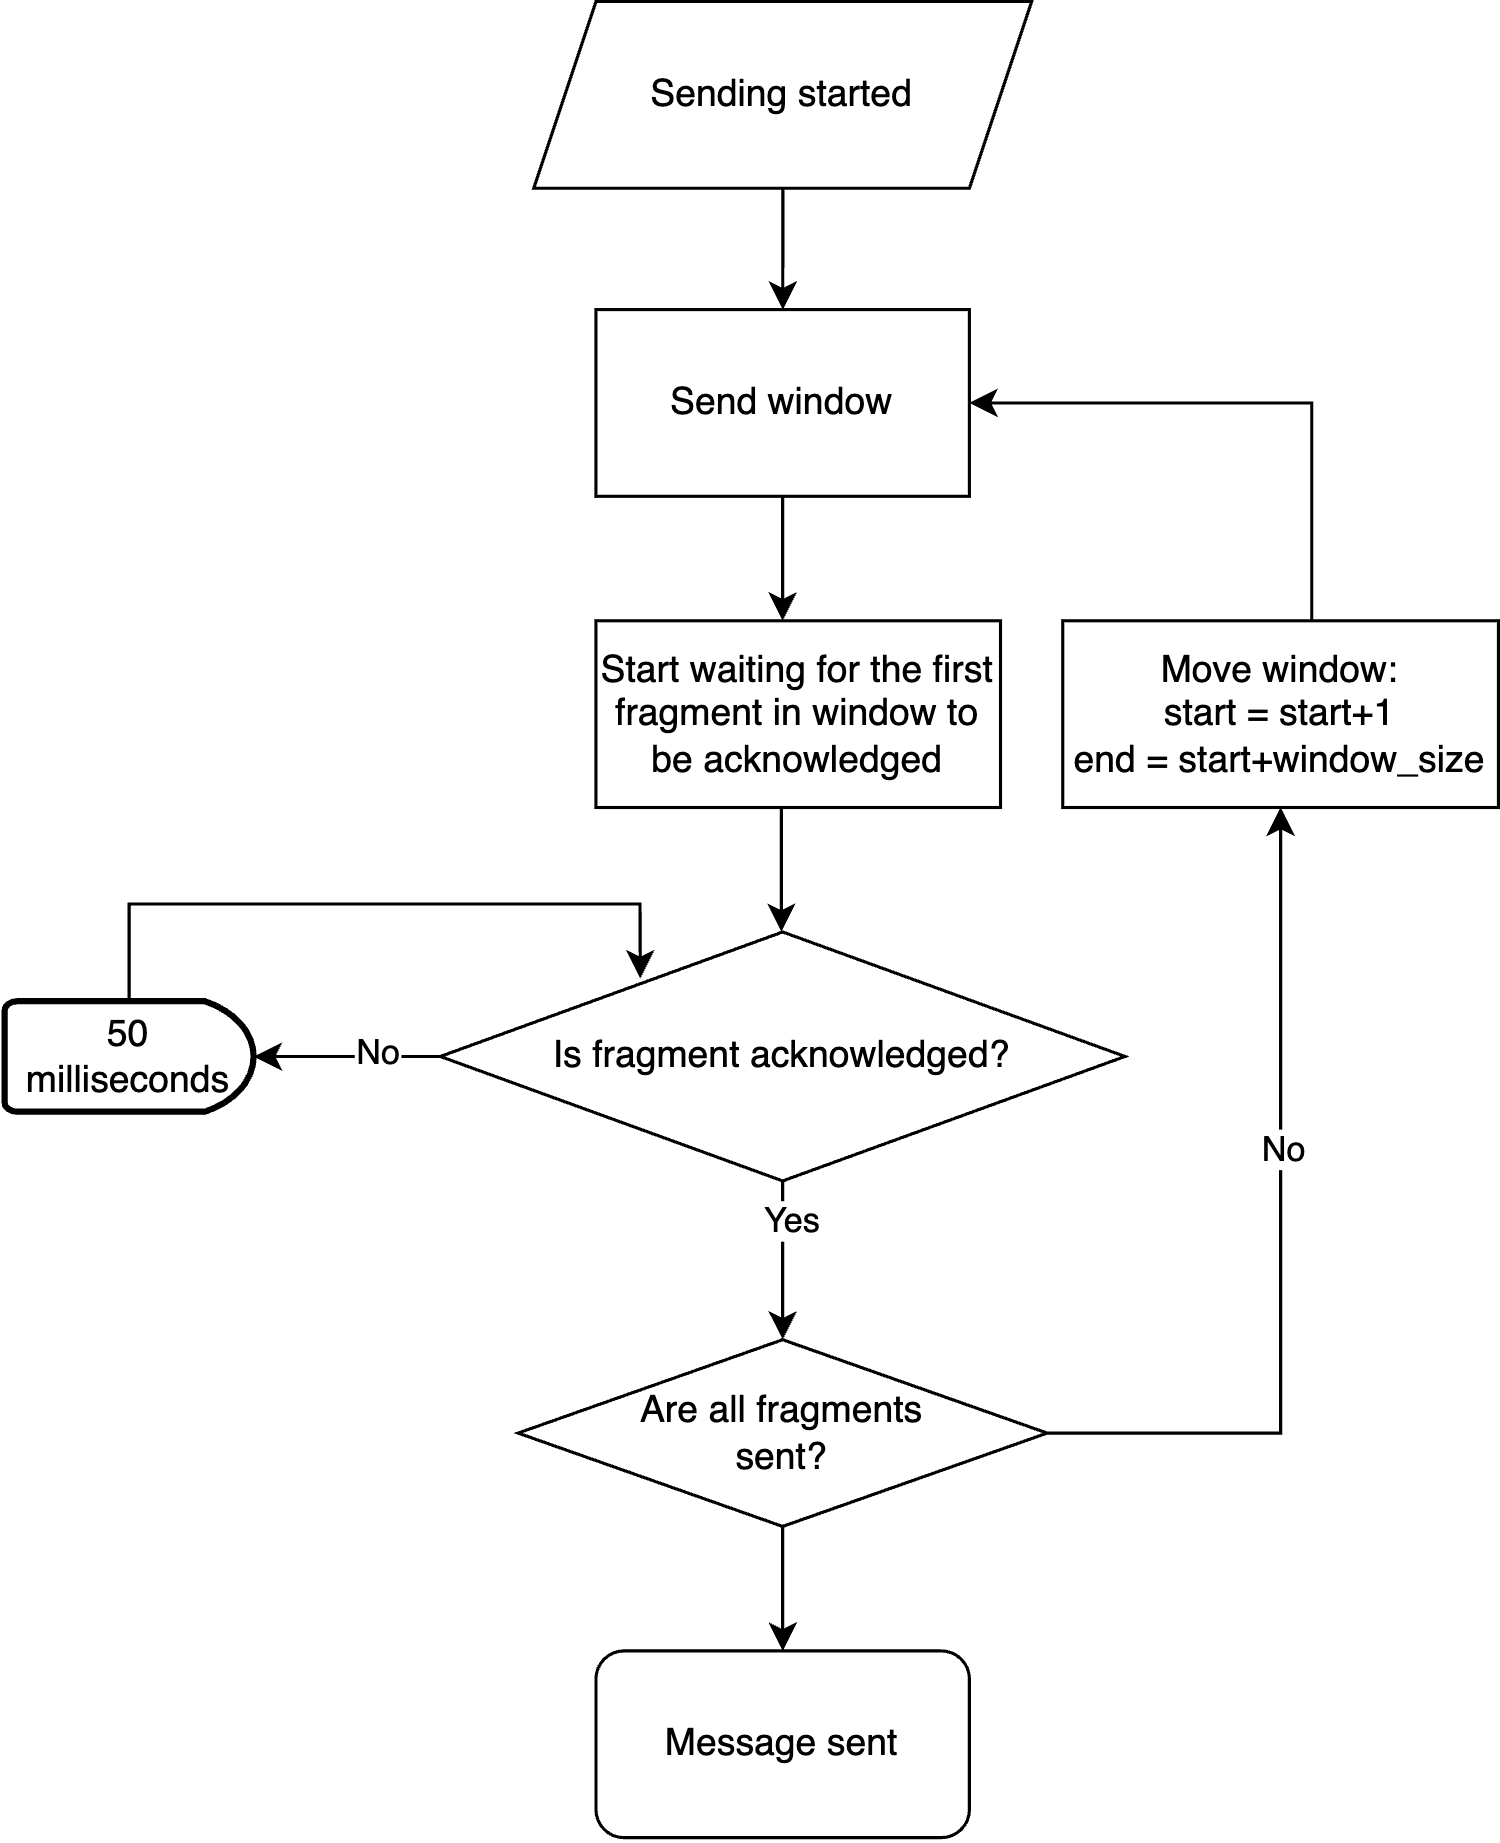
\includegraphics[width=\textwidth]{images/sendingp.png}
    \caption{Sending fragments (for simplicity does not include window size updates and resending fragments, these operations are on separate diagrams)}
    \label{fig:mesh1}
\end{figure}

\begin{figure}[!h]
    \centering
    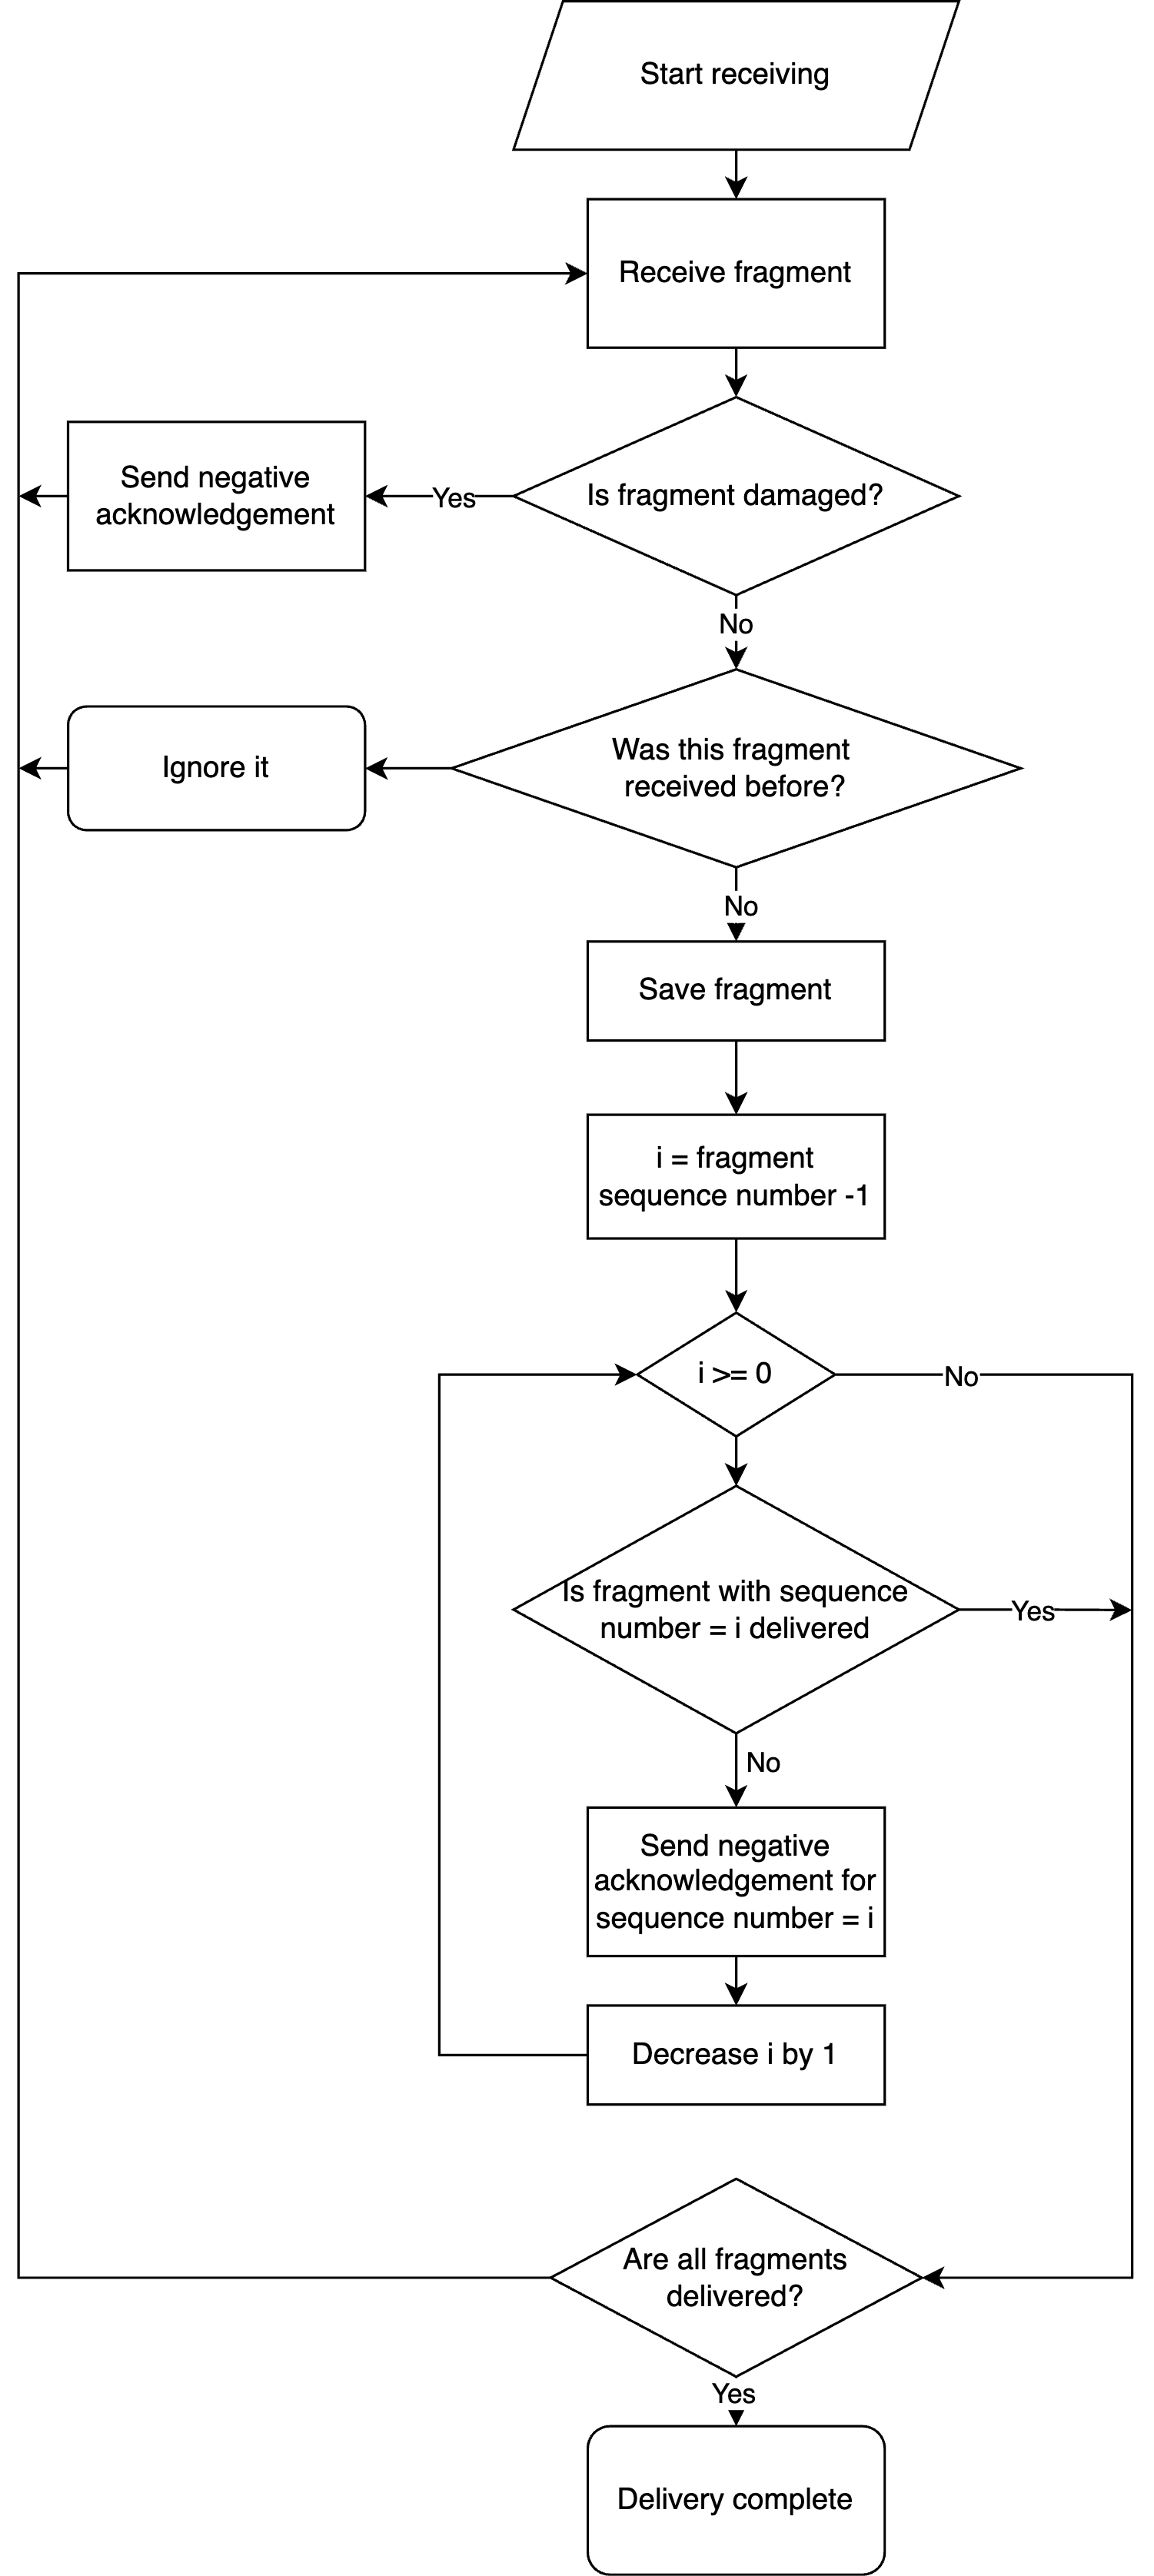
\includegraphics[width=0.7\textwidth]{images/receiving.png}
    \caption{Receiving fragments}
    \label{fig:mesh2}
\end{figure}



\begin{figure}[!h]
    \centering
    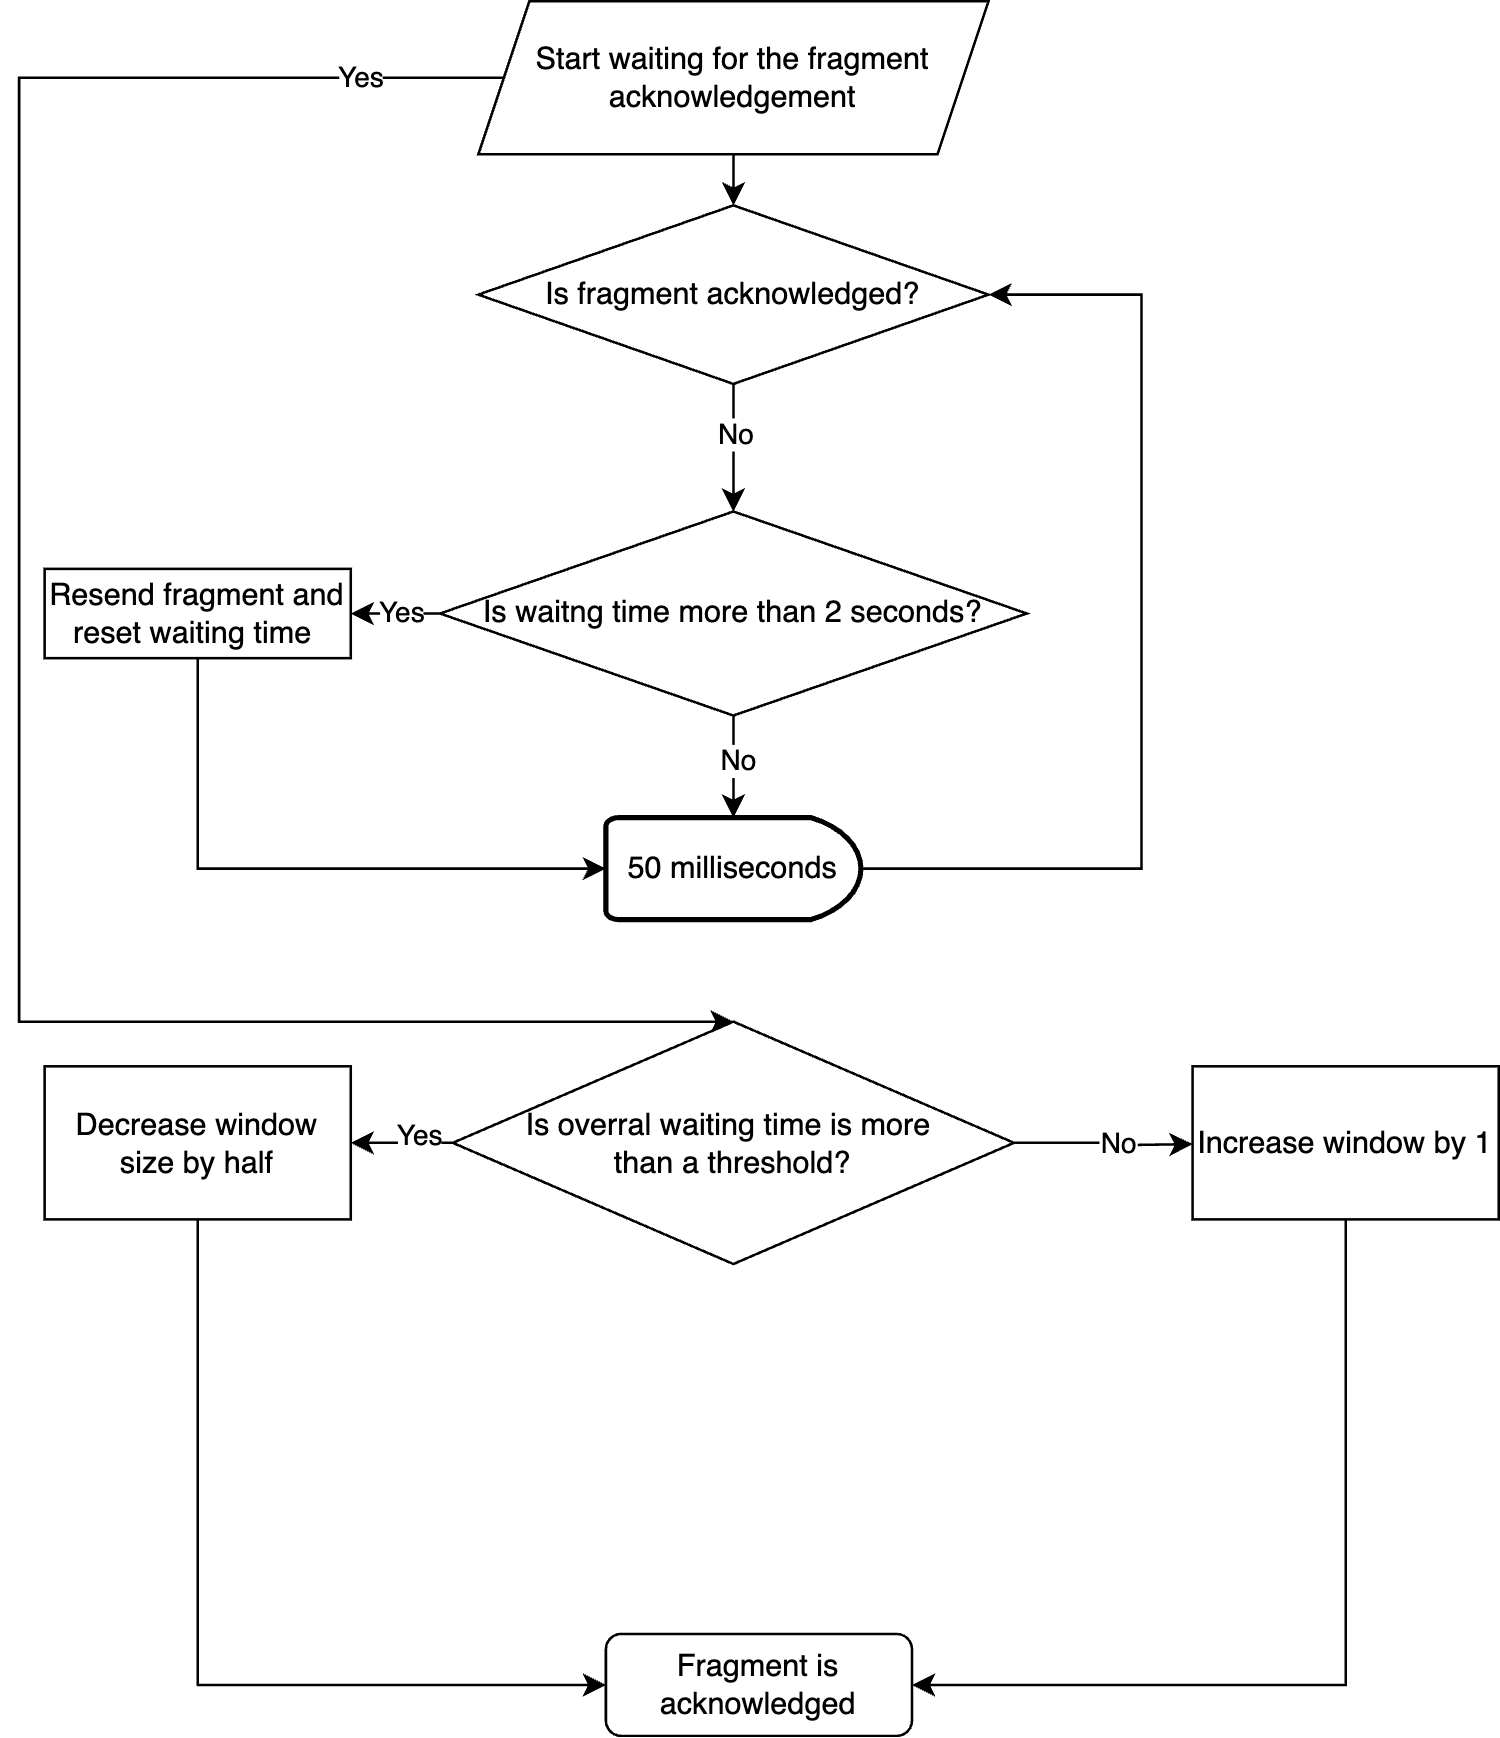
\includegraphics[width=\textwidth]{images/windowmanage.png}
    \caption{Window size management}
    \label{fig:mesh2}
\end{figure}

\begin{figure}[!h]
    \centering
    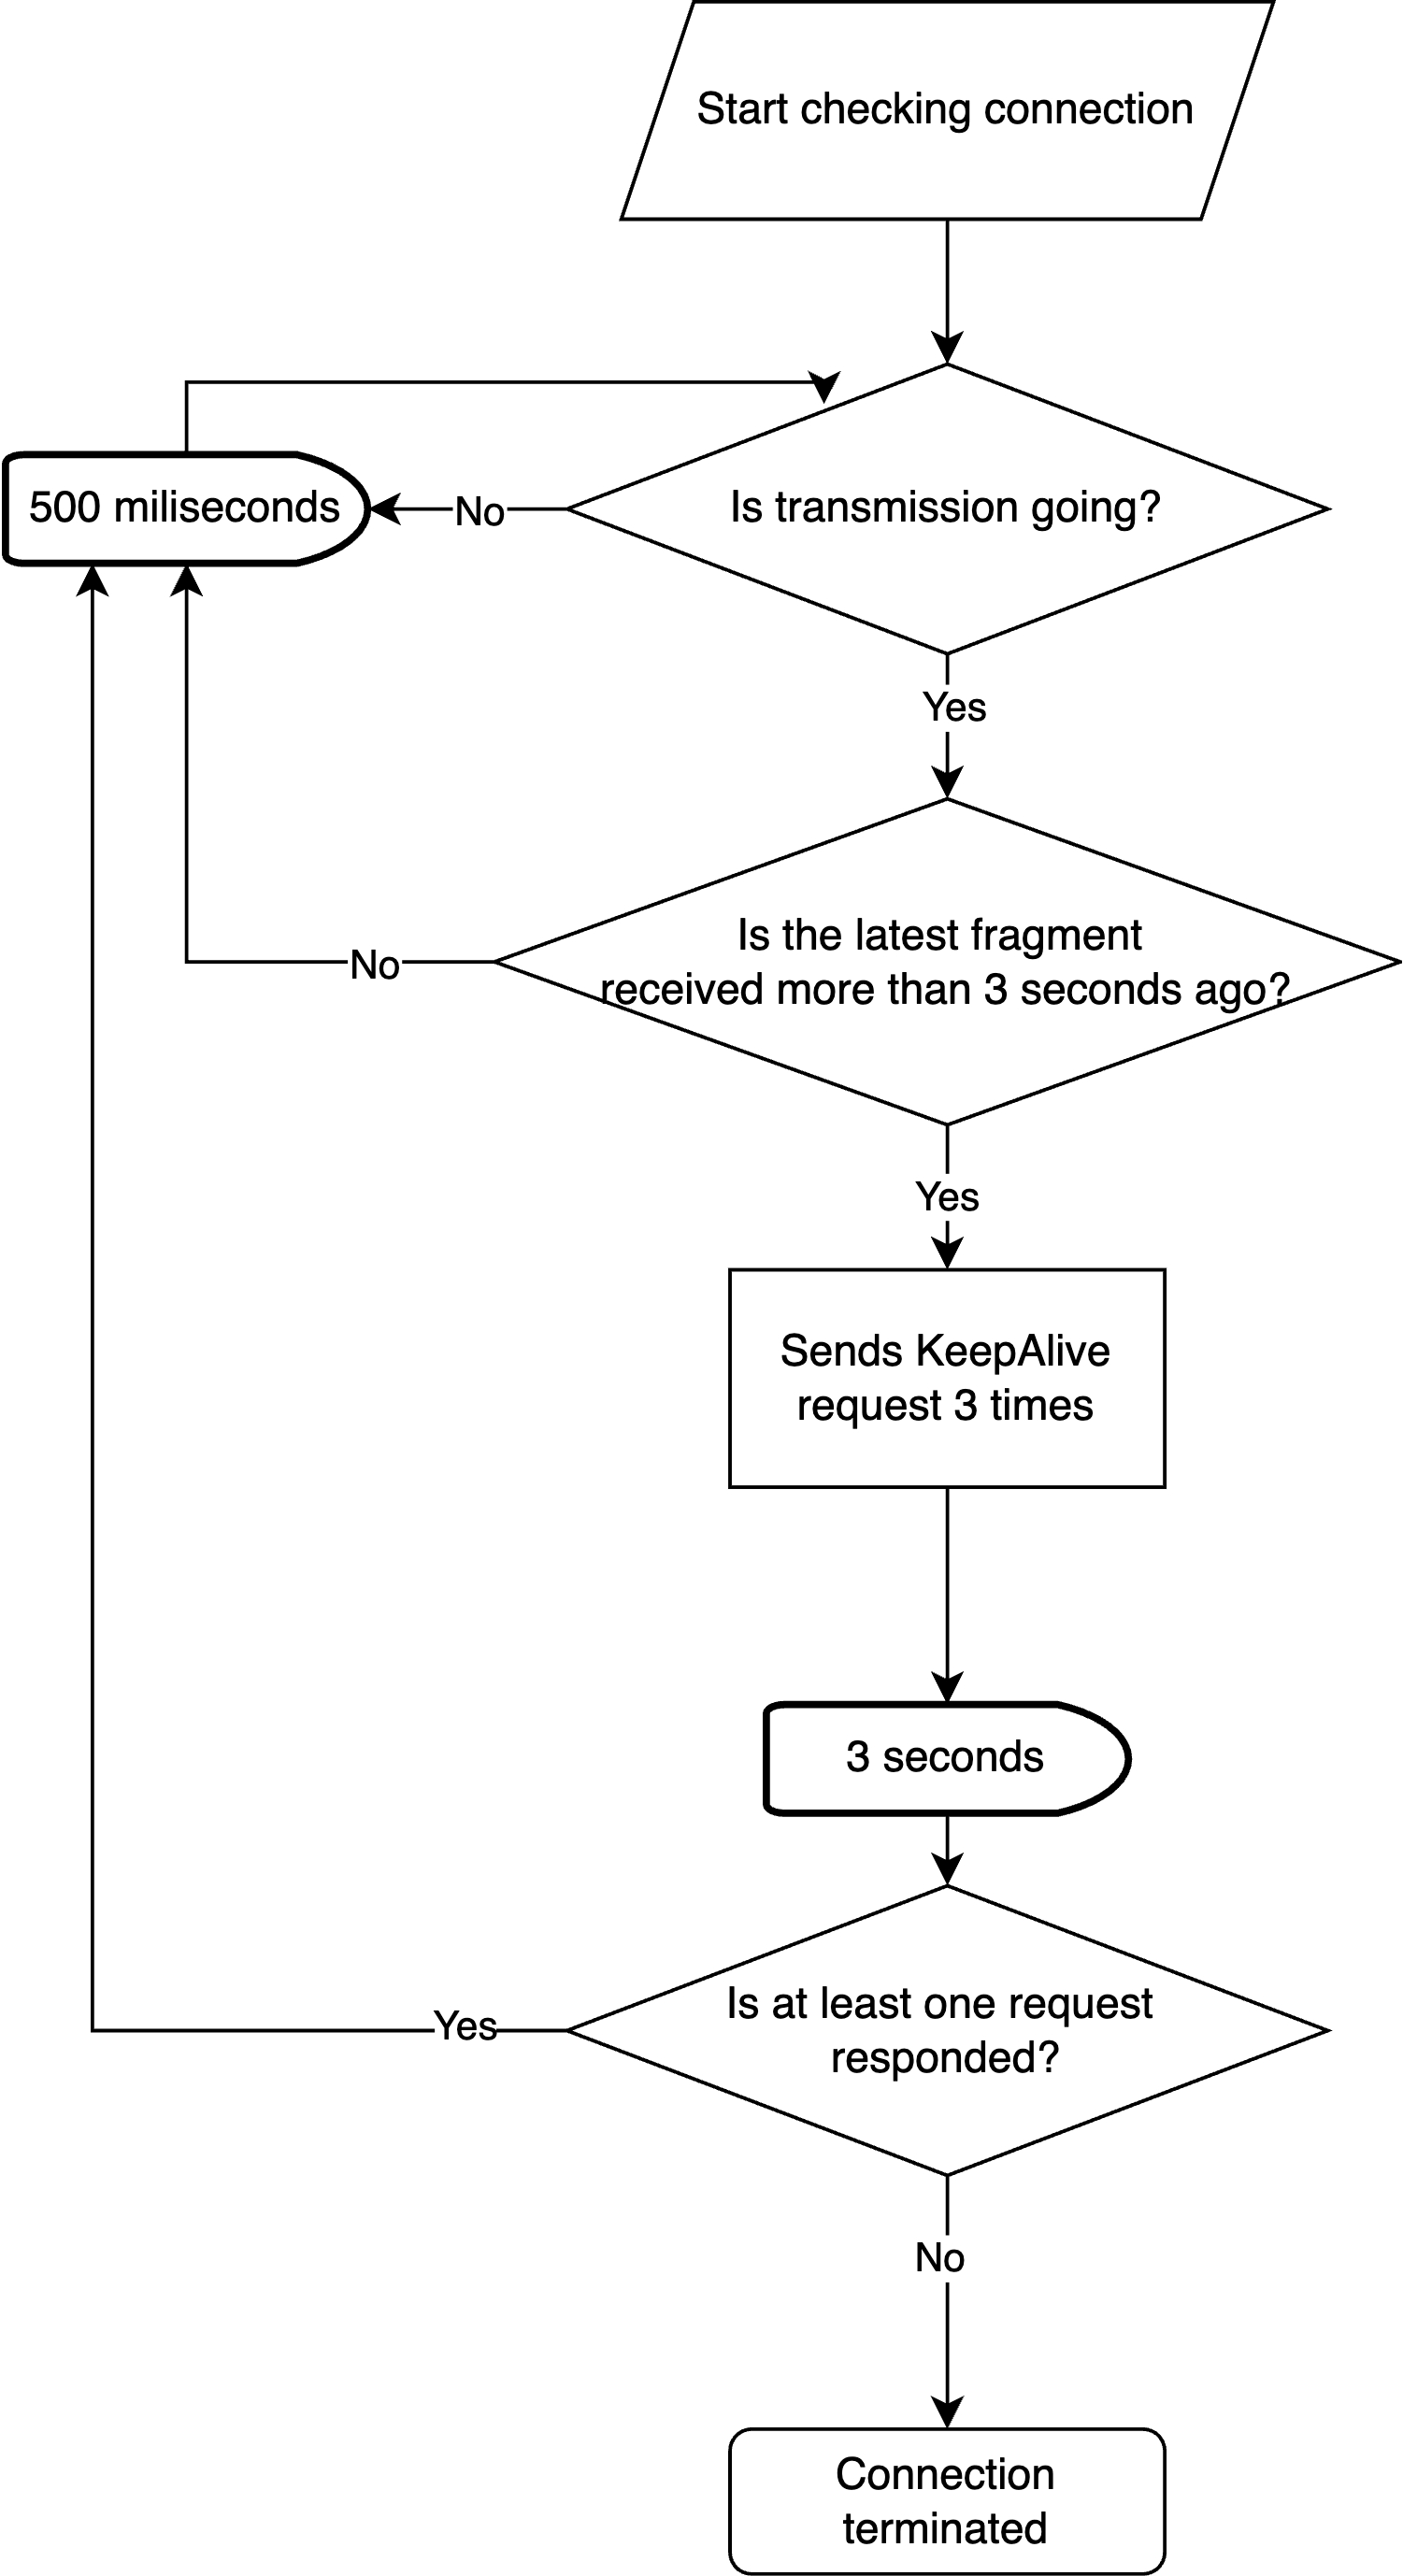
\includegraphics[width=0.75\textwidth]{images/trkeepalive.png}
    \caption{Keeping connection alive when transmitting}
    \label{fig:mesh2}
\end{figure}

\begin{figure}[!h]
    \centering
    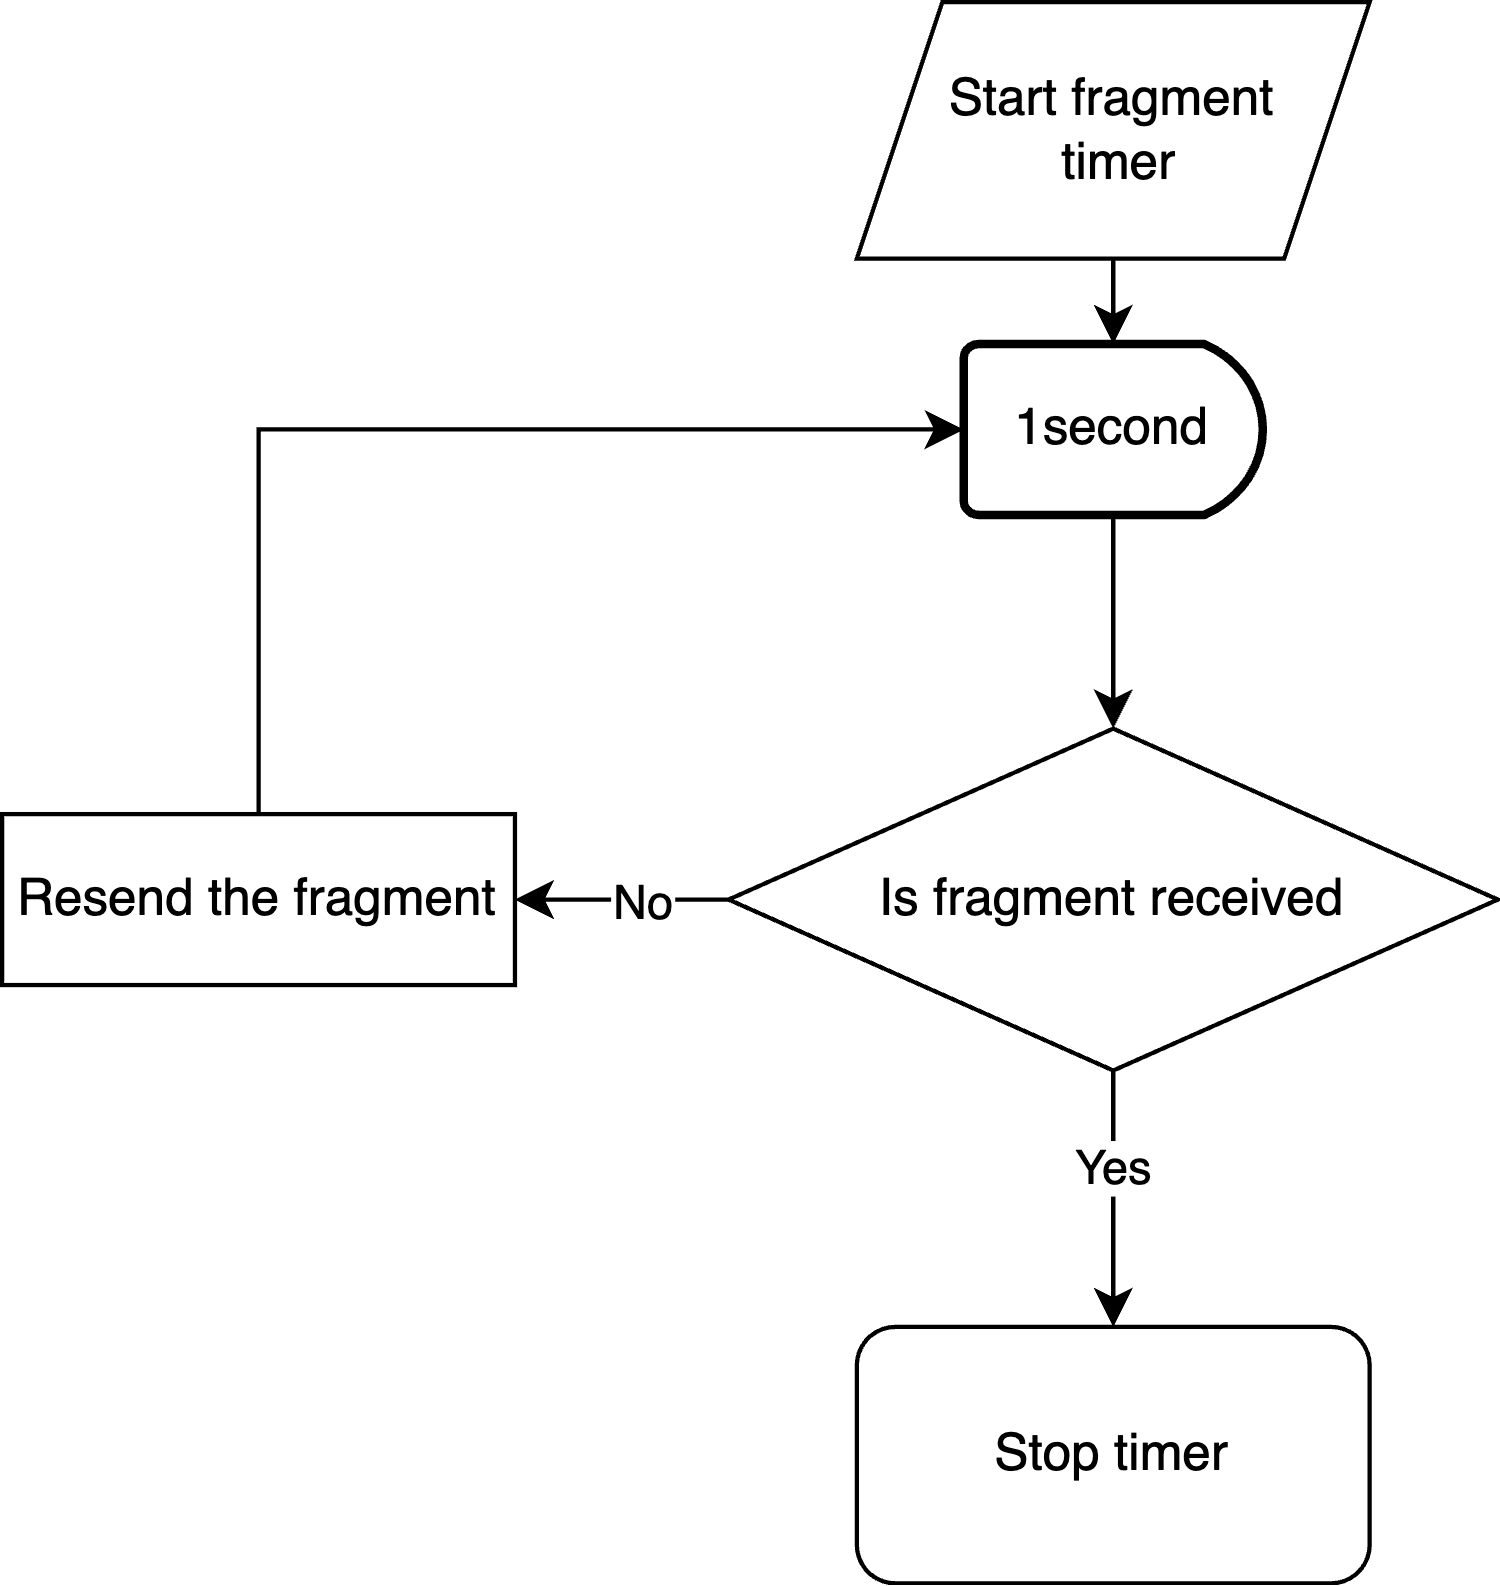
\includegraphics[width=0.75\textwidth]{images/resend.png}
    \caption{Resending fragments}
    \label{fig:mesh2}
\end{figure}

\end{document}
